\clearpage 

\section{Scale Factors and Systematic Uncertainties}\label{systematics}
%%%%
%%%%\subsection{Higher-order QCD and electroweak correction factors}
%%%%
%%%%The transfer factors to the signal regions are defined by taking ratios between the signal and control regions of the relevant MC distributions ($Z,W$+jets). 
%%%%Due to a limited number of simulated events after the tight analysis selection, leading-order MC samples are used for these processes. 
%%%%To correct for next-to-leading-order QCD effects, an event weight is derived as a function of the generator boson $\PT$ ($\PT^V$). 
%%%%A detailed description of these correction factors and the associated uncertainties is given in \cite{CMS_AN_2016-195}.
%%%%These factors are derived using privately produced samples, a description of which follows:
%%%%\begin{itemize}
%%%% \item {\bf W and Z plus jets:} The samples were made using \textsc{amc@nlo}~\cite{MADGRAPH} at NLO in QCD. 
%%%%                                We allow for 0, 1, or 2 extra partons which are matched to a \textsc{pythia} 8.2 parton by the FxFx algorithm~\cite{Frederix:2012ps}. 
%%%%                                The parton distribution function set used was NNPDF 3.0 with 5 flavors.
%%%%\end{itemize}
%%%%To derive the event weights, a ratio is taken between the NLO QCD $\PT^V$ distribution and the LO $\PT^V$ distribution. These weights are then applied to the relevant leading-order samples.
%%%%
%%%%%
%%%%
%%%%In addition to the NLO QCD factor described above, an additional correction is applied to account for higher-order EWK effects which reduce the cross-section at high $\PT^V$.  
%%%%These are derived in Refs.~\cite{Kallweit:2014xda} and \cite{Kallweit:2015fta}. 
%%%%
%%%%The higher-order corrections are shown as a function of $\PT^V$ in Figure~\ref{fig:nlo_corrections}.
%%%%
%%%%\begin{figure}[htbp]
%%%%  \begin{center}
%%%%    \subfigure[$W$+jets]{
%%%%      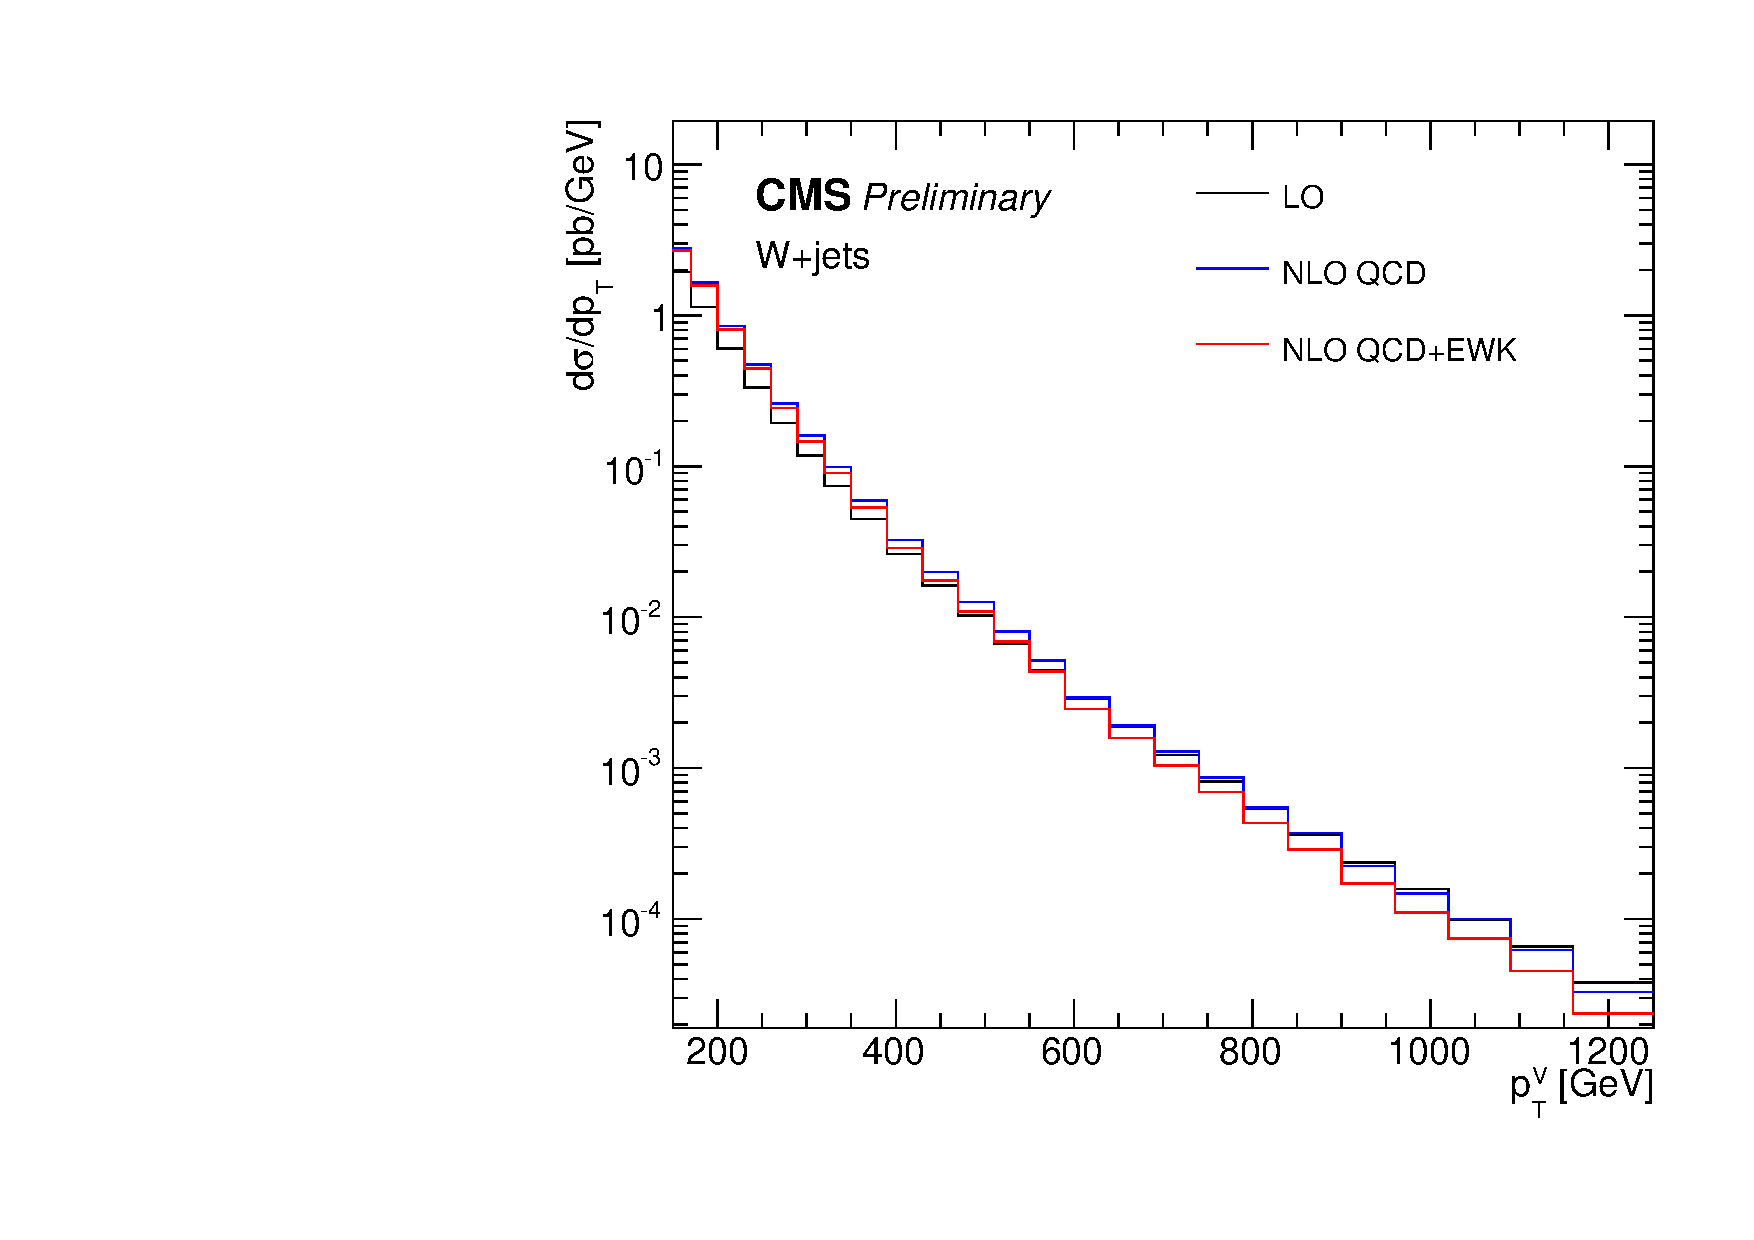
\includegraphics[width=0.49\textwidth]{figures/kfactors/W.pdf}
%%%%      \label{fig:nlo_w}
%%%%    }
%%%%    \subfigure[$Z$+jets]{
%%%%      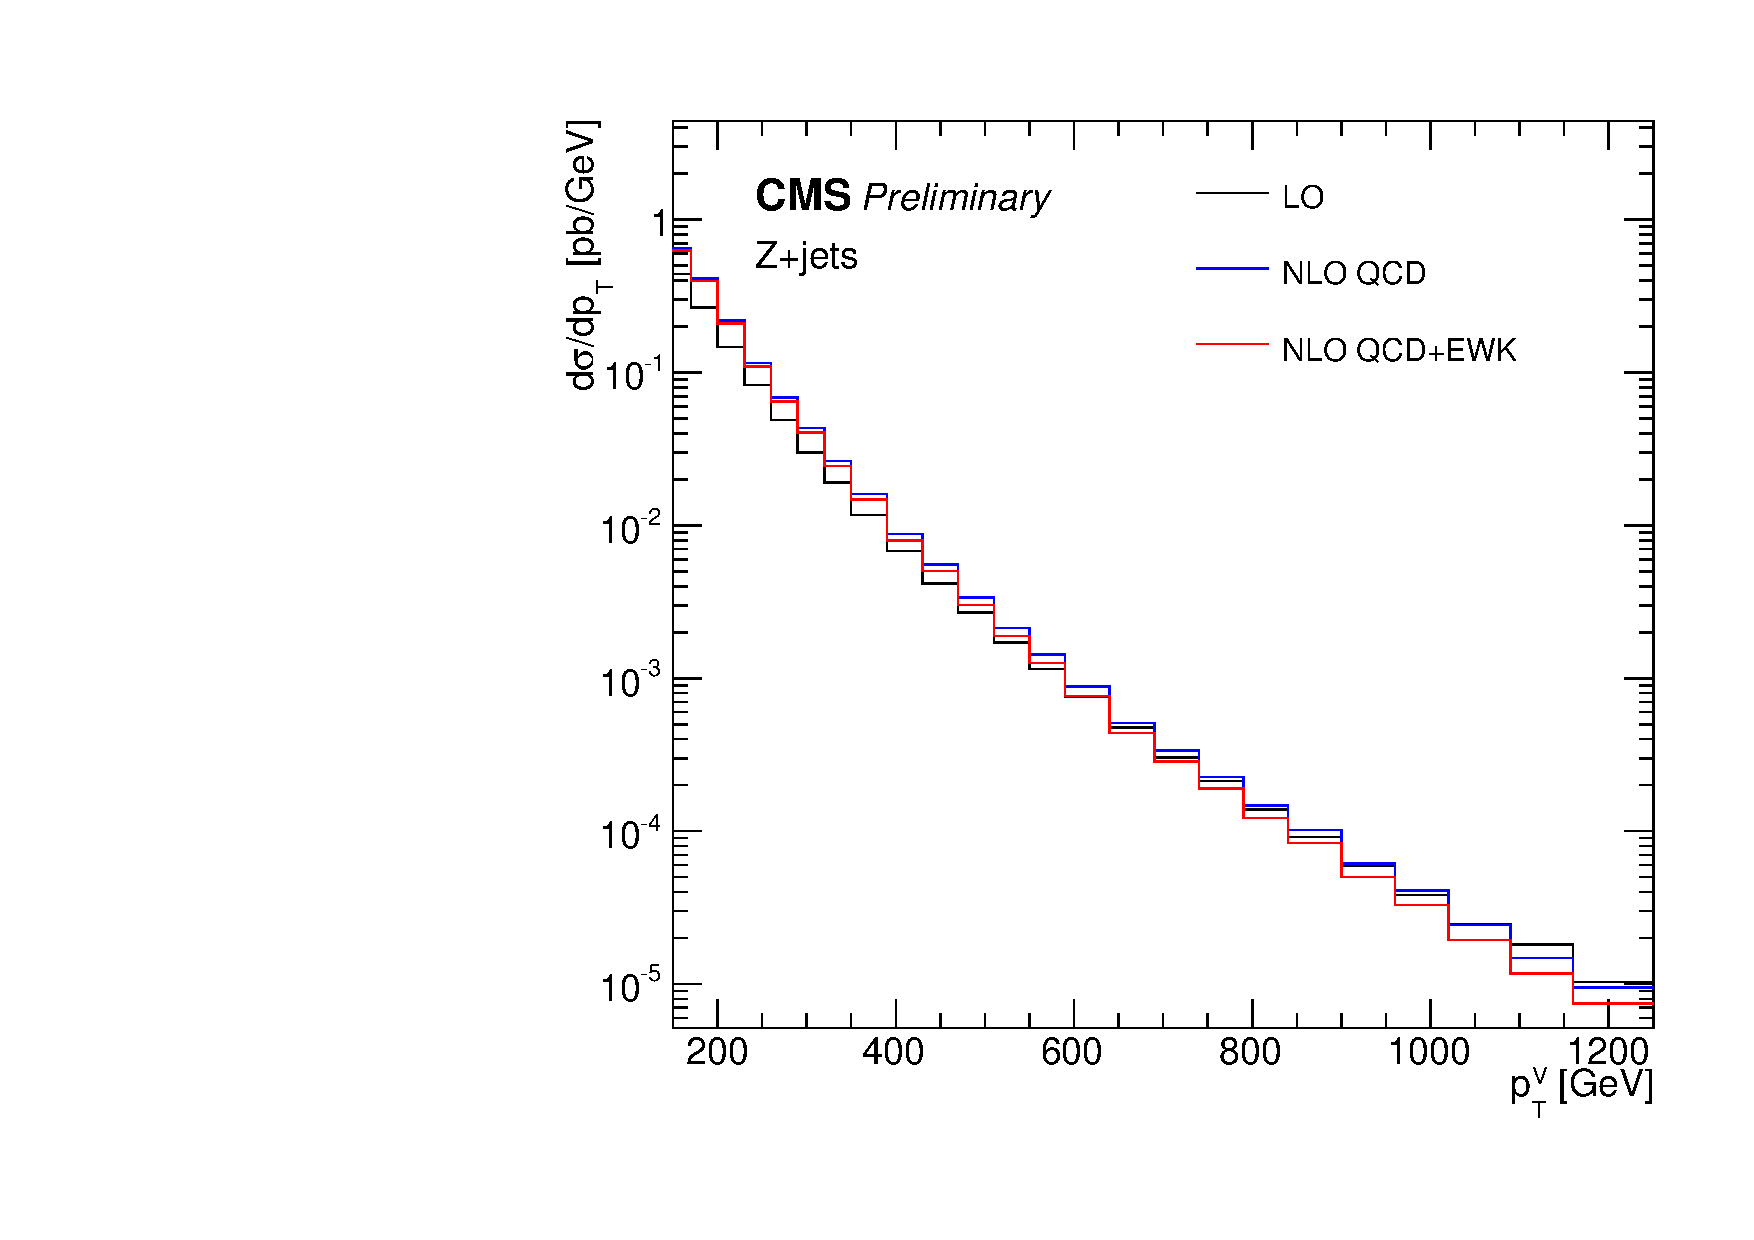
\includegraphics[width=0.49\textwidth]{figures/kfactors/Z.pdf}
%%%%      \label{fig:nlo_z}
%%%%    }
%%%%    \caption{
%%%%      Higher-order corrections for $V$+jets Monte Carlo samples
%%%%    }
%%%%    \label{fig:nlo_corrections}
%%%%  \end{center}
%%%%\end{figure}
%%%%
%%%%PDF uncertainties are propagated when the event is generated and the shifted scale factors are computed using the corresponding shifted $\PT^V$ distributions.
%%%%The uncertainty on the nominal SF is taken as the RMS of the shifted SFs.
%%%%A similar approach is taken for the uncertainty from the higher-order QCD corrections.
%%%%The factorization and renormalization scales are allowed to vary by $0.5$ and $2$. 
%%%%A comparison of these uncertainties is in Figure~\ref{fig:qcduncertainty}.
%%%%
%%%%It should be noted that the monojet analysis~\cite{CMS_AN_2016-473} has migrated to a less conservative set of QCD uncertainties.
%%%%However, these uncertainties were derived for a very specific phase-space.
%%%%The additional requirements on a massive fatjet (which effectively requires more narrow jets in the event) can move significantly away from the monojet regime.
%%%%Since the new prescription has not yet been validated for the phase-space used in this analysis, we continue to use a more conservative uncertainty scheme.
%%%%
%%%%\begin{figure}[htbp]
%%%%  \begin{center}
%%%%      \centering
%%%%      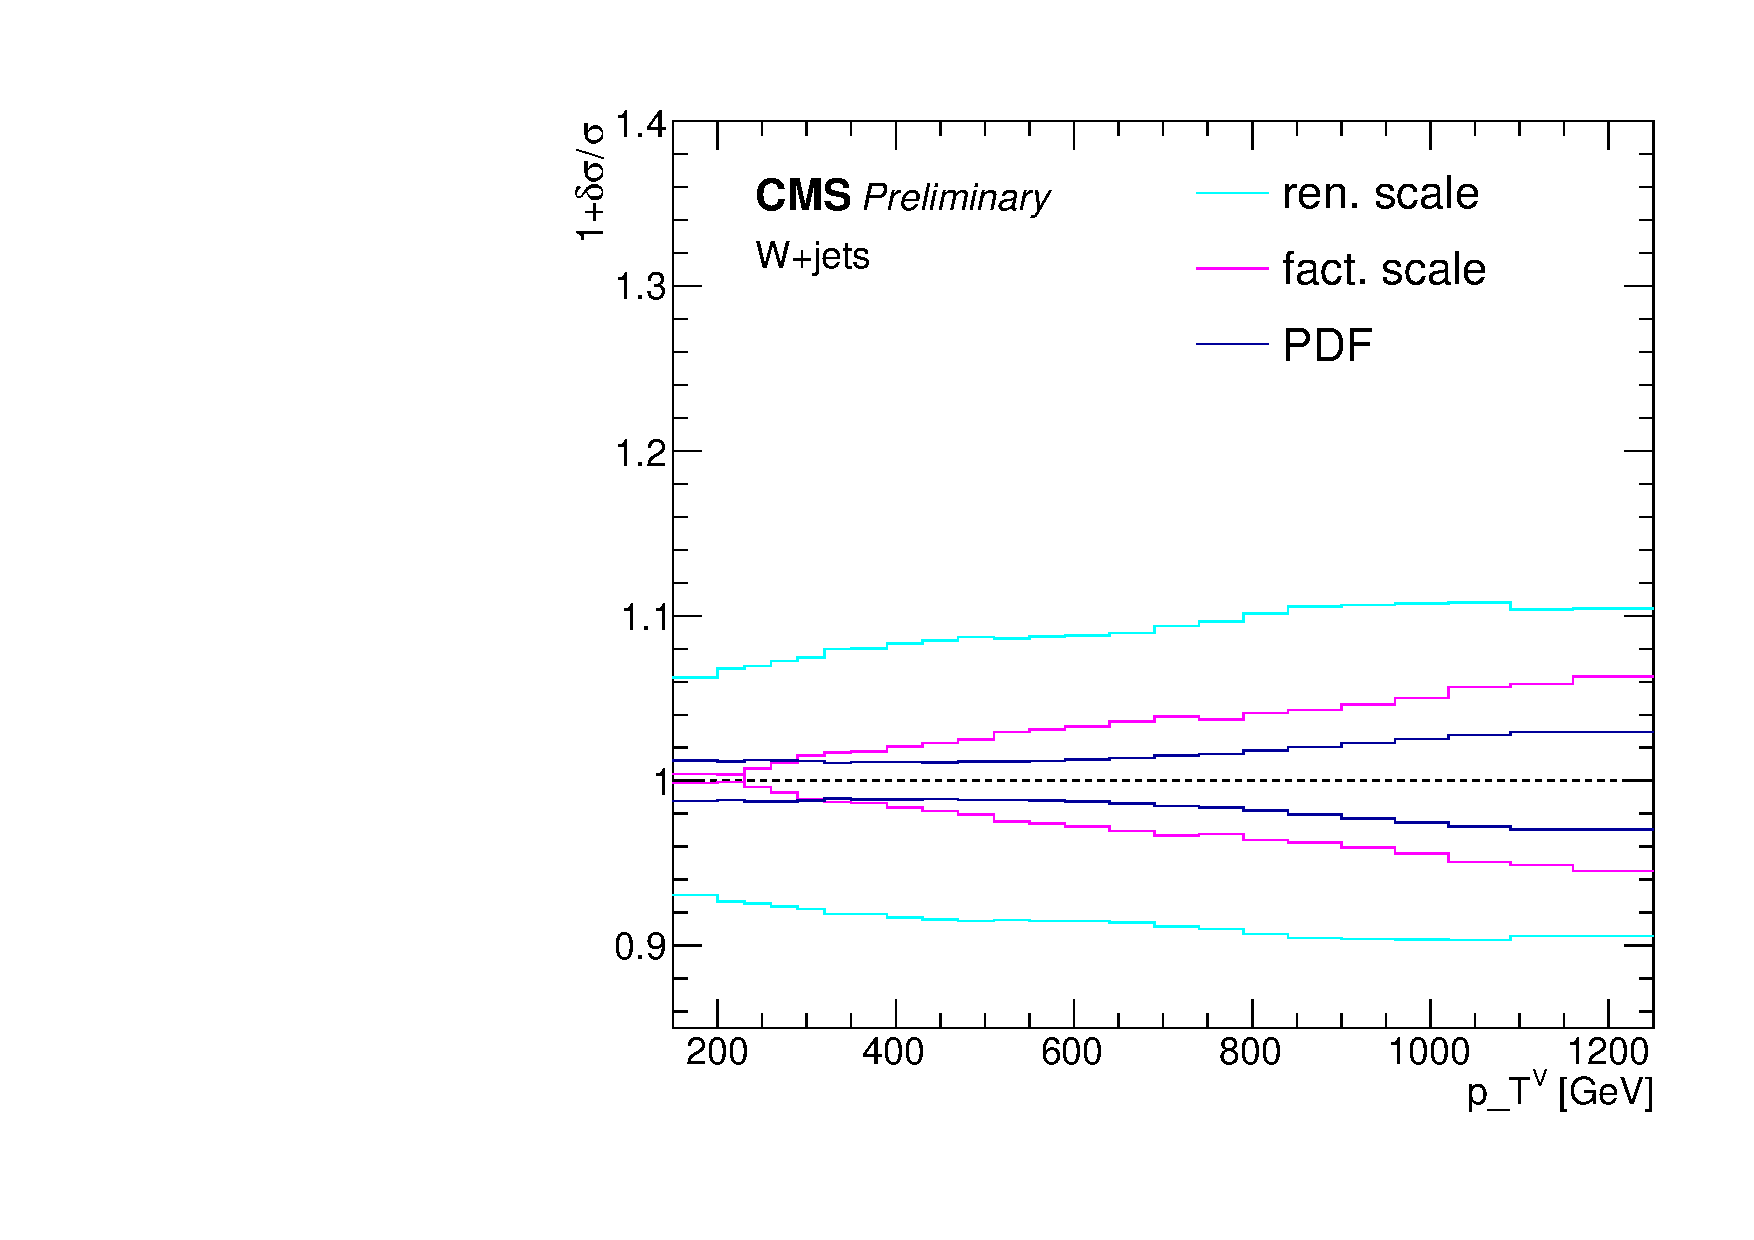
\includegraphics[width=.49\textwidth]{figures/kfactors/uncertW.pdf}
%%%%      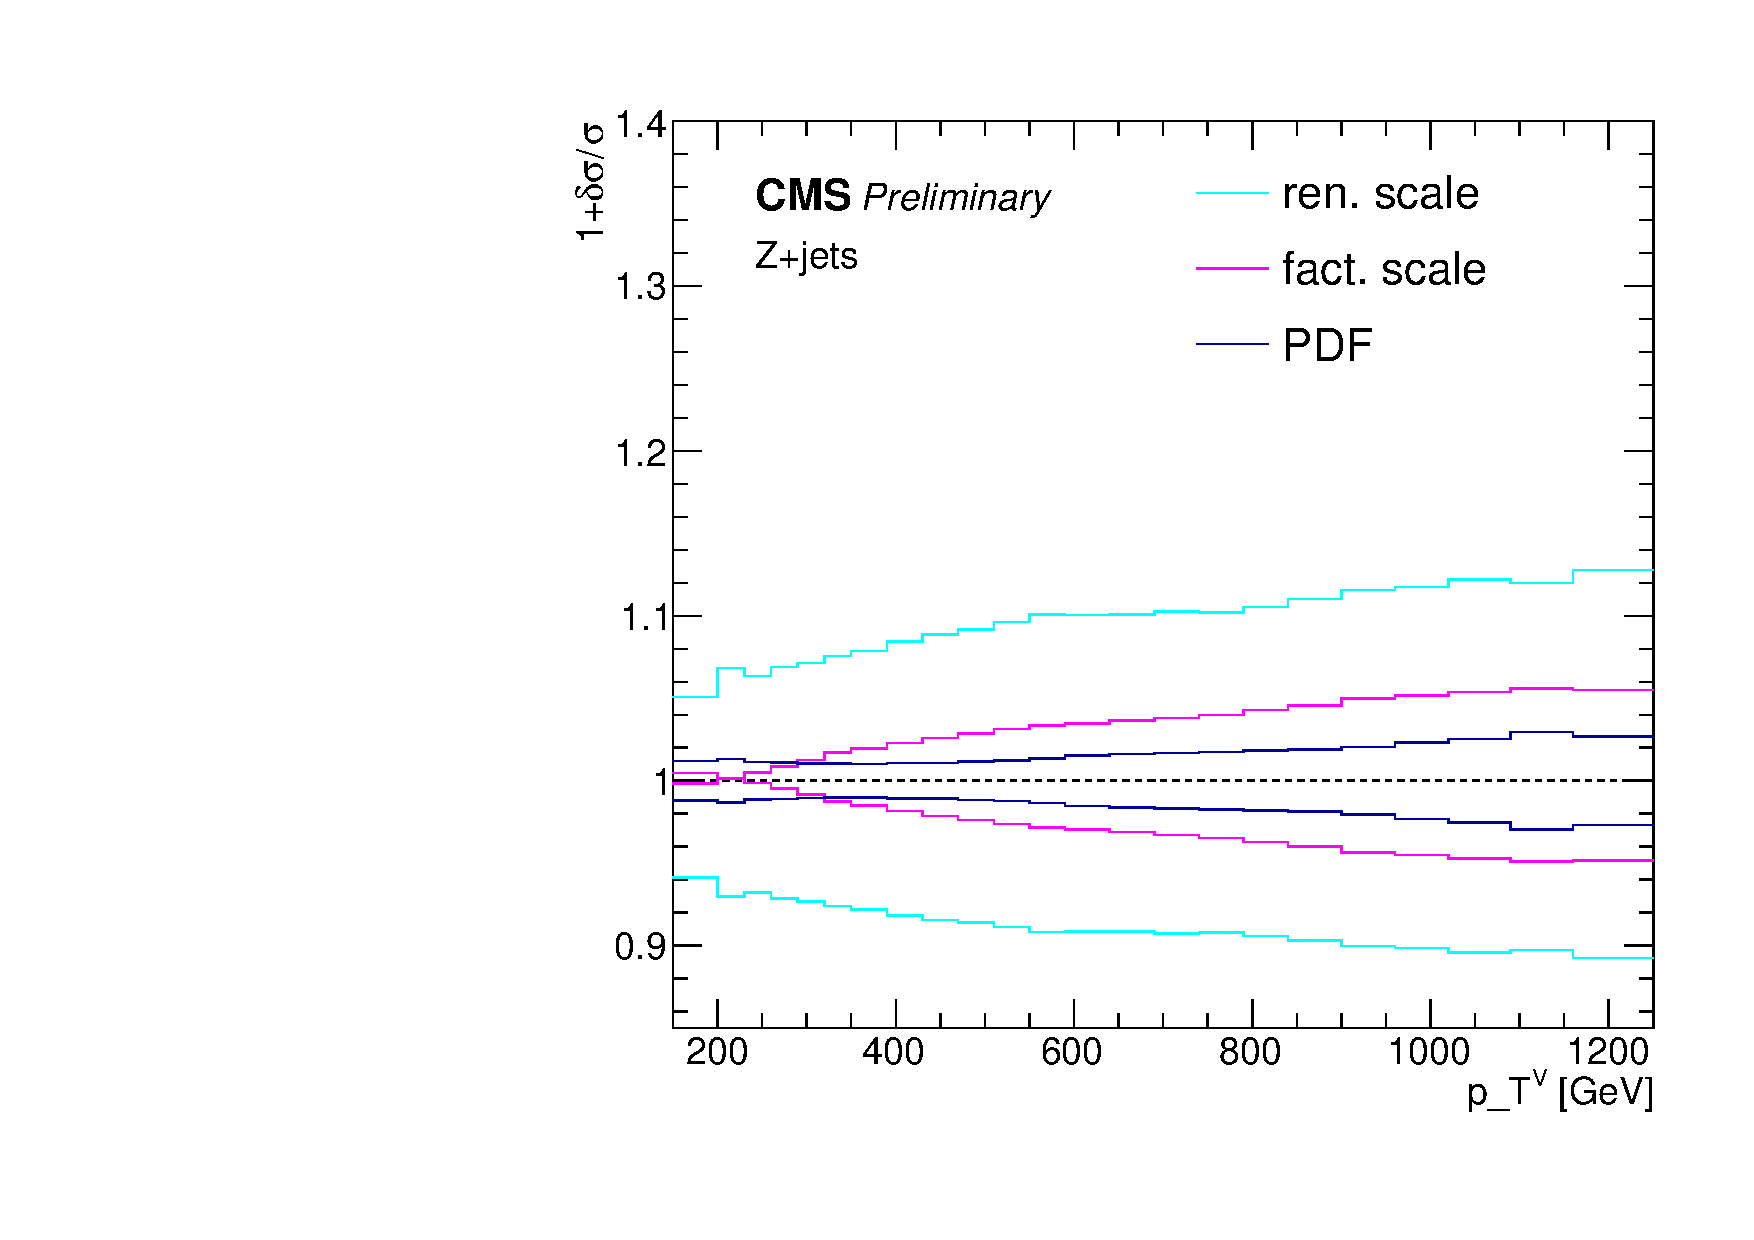
\includegraphics[width=.49\textwidth]{figures/kfactors/uncertZ.pdf}\\
%%%%    \caption{
%%%%      Comparison of PDF and QCD scale uncertainties on the $\PT^{V}$
%%%%      distributions.
%%%%    }
%%%%    \label{fig:qcduncertainty}
%%%%  \end{center}
%%%%\end{figure}
%%%%
%%%%Finally, the uncertainty due to higher-order EWK corrections is considered, as is done in~\cite{CMS_AN_2016-473}.
%%%%There are three sources of uncertainty:
%%%%\begin{itemize}
%%%%  \item Corrections beyond NNLO EWK due to Sudakov logs. This uncertainty must be correlated across \pt and between $W,Z$. This is labelled $\delta^1_\mathrm{EW}$ in~\cite{CMS_AN_2016-473}.
%%%%  \item Missing NNLO EWK effects. These are uncorrelated between each process ($W,Z$) and labelled $\delta^2_\mathrm{EW}$.
%%%%  \item Difference between NLL Sudakov and exponentiating NLO EWK is considered an uncertainty on the NNLO EWK correction. These are also uncorrelated between each process ($W,Z$) and labelled $\delta^3_\mathrm{EW}$.
%%%%\end{itemize}
%%%%
\subsection{Heavy-flavor fraction uncertainty}\label{sec:hffrac}
When using our control regions to constrain the signal region, we rely on knowing the heavy-flavor fraction of the backgrounds in order to be able to accurately build transfer factors between regions with different $b$-tagging requirements.
Unfortunately, the heavy-flavor fraction is not well-modeled from theory.
Therefore, an estimation on the uncertainty is made using experimental results.
CMS has measured the differential cross-section of $W$+jets as a function of $N_\text{jets}$ \cite{CMS-PAS-SMP-12-023}. 
From this study, we make the conservative estimate that the uncertainty on the cross-section of $W$+fat jet is less than $20\%$ (Figure~\ref{fig:wnjets}). 

\begin{figure}[htbp]
  \centering
  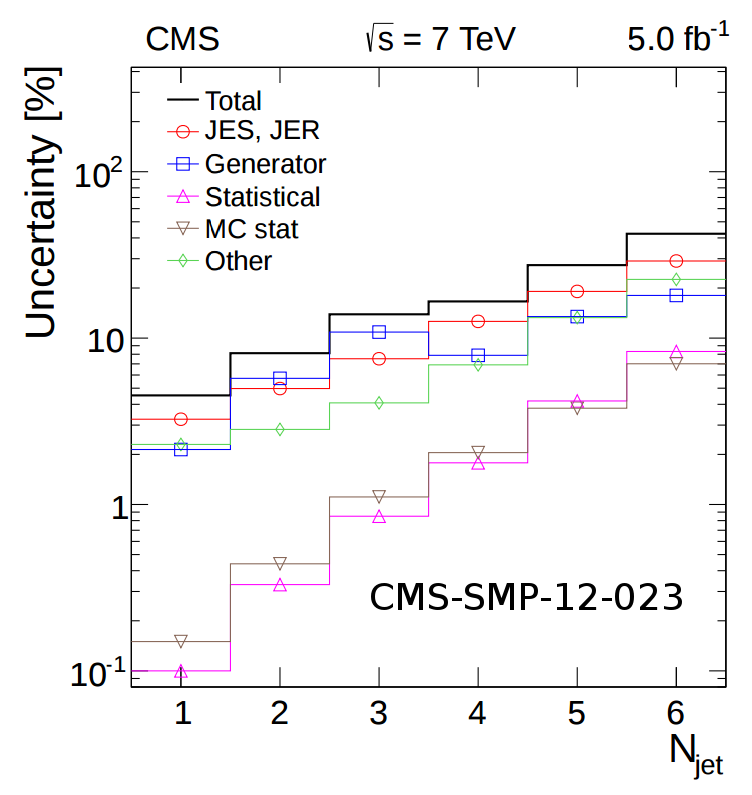
\includegraphics[width=0.5\textwidth]{figures/wnjets.png}
  \caption{Figure from Ref.~\cite{CMS-PAS-SMP-12-023} showing uncertainty in $W+$jets production as a function of $N_\text{jets}$. To estimate an uncertainty on the production of $W$+fat jet, we look at the $N_\text{jets}=2,3$ bins.}
  \label{fig:wnjets}
\end{figure}

Next, using CMS measurements of $W+c$ \cite{CMS-PAS-SMP-13-149} and $W+b\bar{b}$ \cite{CMS-PAS-SMP-12-026} production, we extract the following uncertainties on heavy-flavor production:

\begin{equation}
  \frac{\delta\sigma(W+c, W\rightarrow \ell\nu)}{\sigma(W+c, W\rightarrow \ell\nu)} = \frac{7.65~\text{pb}}{107.7~\text{pb}}, \quad \frac{\delta\sigma(W+b\bar{b}, W\rightarrow \ell\nu)}{\sigma(W+b\bar{b}, W\rightarrow \ell\nu)} = \frac{0.206~\text{pb}}{1.06~\text{pb}}
\end{equation}
The uncertainties are then propagated as follows:

\begin{align*}
  \frac{\delta\sigma(W+\text{HF})}{\sigma(W+\text{fat jet})} &= \left[ \left(\frac{\delta\sigma(W+\text{HF})}{\sigma(W+\text{HF})}\right)^2 + \left(\frac{\delta\sigma(W+\text{fat jet})}{\sigma(W+\text{fat jet})}\right)^2  \right]^{1/2} \nonumber\\
            &= \left[ \frac{\delta\sigma(W+c)^2+\delta\sigma(W+b\bar{b})^2}{\left(\sigma(W+c) + \sigma(W+b\bar{b})\right)^2} + \left(\frac{\delta\sigma(W+\text{fat jet})}{\sigma(W+\text{fat jet})}\right)^2  \right]^{1/2}
\end{align*}
Using the values discussed above, we arrive at:

\begin{equation}
  \frac{\delta\sigma(W+\text{HF}, W\rightarrow \ell\nu)}{\sigma(W+\text{fat jet}, W\rightarrow \ell\nu)} \approx 0.21
\end{equation}

A similar calculation is done for $Z$+jets.
First, we estimate the uncertainty $Z+$fat jet production \cite{CERN-PH-EP-2014-205} as $15\%$ using Figure~\ref{fig:znjets}.

\begin{figure}[htbp]
  \centering
  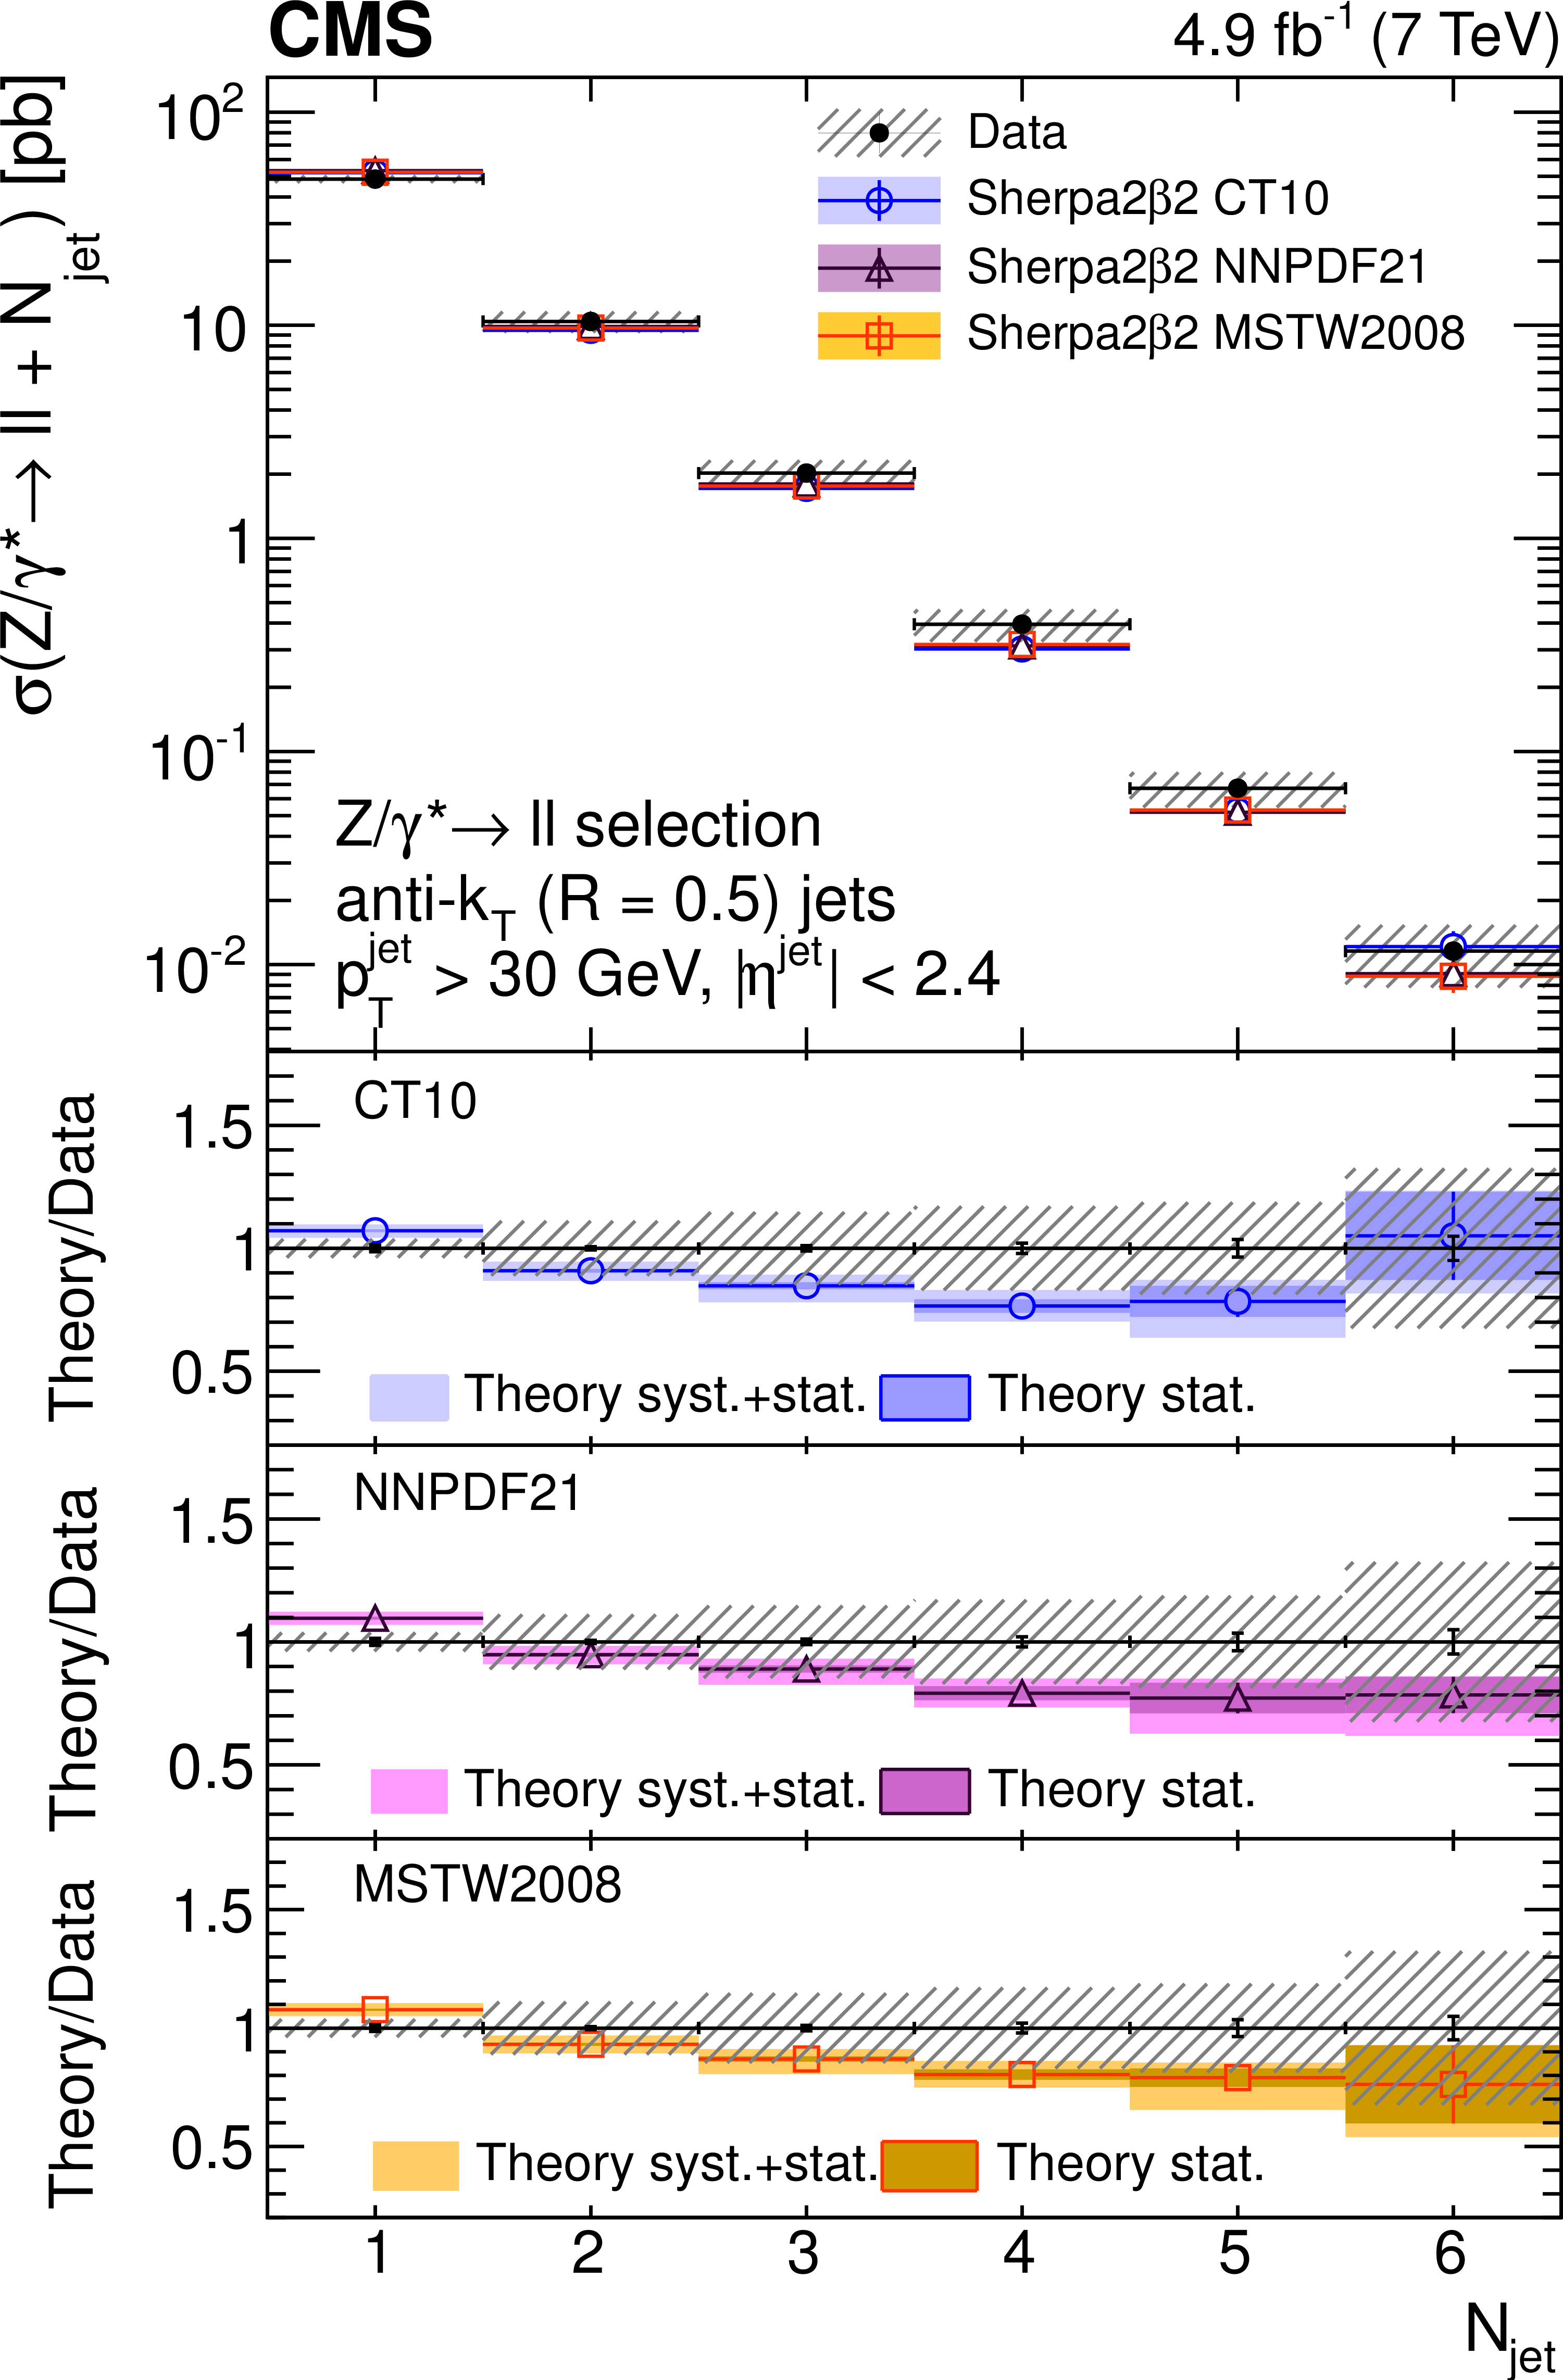
\includegraphics[width=0.4\textwidth]{figures/znjets.png}
  \caption{Figure from Ref.~\cite{CERN-PH-EP-2014-205} showing uncertainty in $Z+$jets production as a function of $N_\text{jets}$. To estimate an uncertainty on the production of $Z$+fat jet, we look at the $N_\text{jets}=2,3$ bins.}
  \label{fig:znjets}
\end{figure}

Then, from \cite{CERN-PH-EP-2014-005}, we get the the uncertainty on $Z+b(b)$ production as:

\begin{equation}
  \frac{\delta\sigma(Z+b(b))}{\sigma(Z+b(b))} = \frac{0.909~\text{pb}}{5.84~\text{pb}}
\end{equation}
The resulting uncertainty on the heavy-flavor fraction is:

\begin{equation}
  \frac{\delta\sigma(Z+\text{HF}, Z\rightarrow \ell\ell)}{\sigma(Z+\text{fat jet}, Z\rightarrow \ell\ell)}  = \left[ \left(\frac{\delta\sigma(Z+\text{HF})}{\sigma(Z+\text{HF})}\right)^2 +  \left(\frac{\delta\sigma(Z+\text{fat jet})}{\sigma(Z+\text{fat jet})}\right)^2 \right]^{1/2} = 0.22
\end{equation}

All HF-fraction uncertainties are then propagated through as rate uncertainties on the respective processes. 
That is, two nuisances are added to the fit: $Z+$HF and $W+$HF.
These nuisances are correlated across the relevant processes in all regions.
Depending on the process and region, the rate uncertainties range from $4\%$ to $5\%$. 


\subsection{$b$-tagging scale factors}\label{sec:btagsfs}

The BTV POG provides scale factors and associated uncertainties for $b$-tagging of narrow jets. 
These object scale factors are propagated into event scale factors for this analysis. 
The associated uncertainties are propagated as two sets of shape variations: narrow jet $b$-tag and narrow jet mis-tag.
The recommendations for the scale factors and uncertainties are from Ref~\cite{TWIKI-BTAG}.

The scale factors and uncertainties provided by the POG largely cover the $p_T$ range probed in this analysis. AK4 jet SFs are provided for $p_T<1000~\GeV$. For jets beyond this $p_T$ range, the recommendation is to use the scale factor from the $p_T$ boundary and double the uncertainty (Ref~\cite{TWIKI-BTAG}). As shown in Figure~\ref{fig:bjetspectra}, very few jets in this analysis extend past these $p_T$ bounds.

\begin{figure}[htbp]
  \centering
  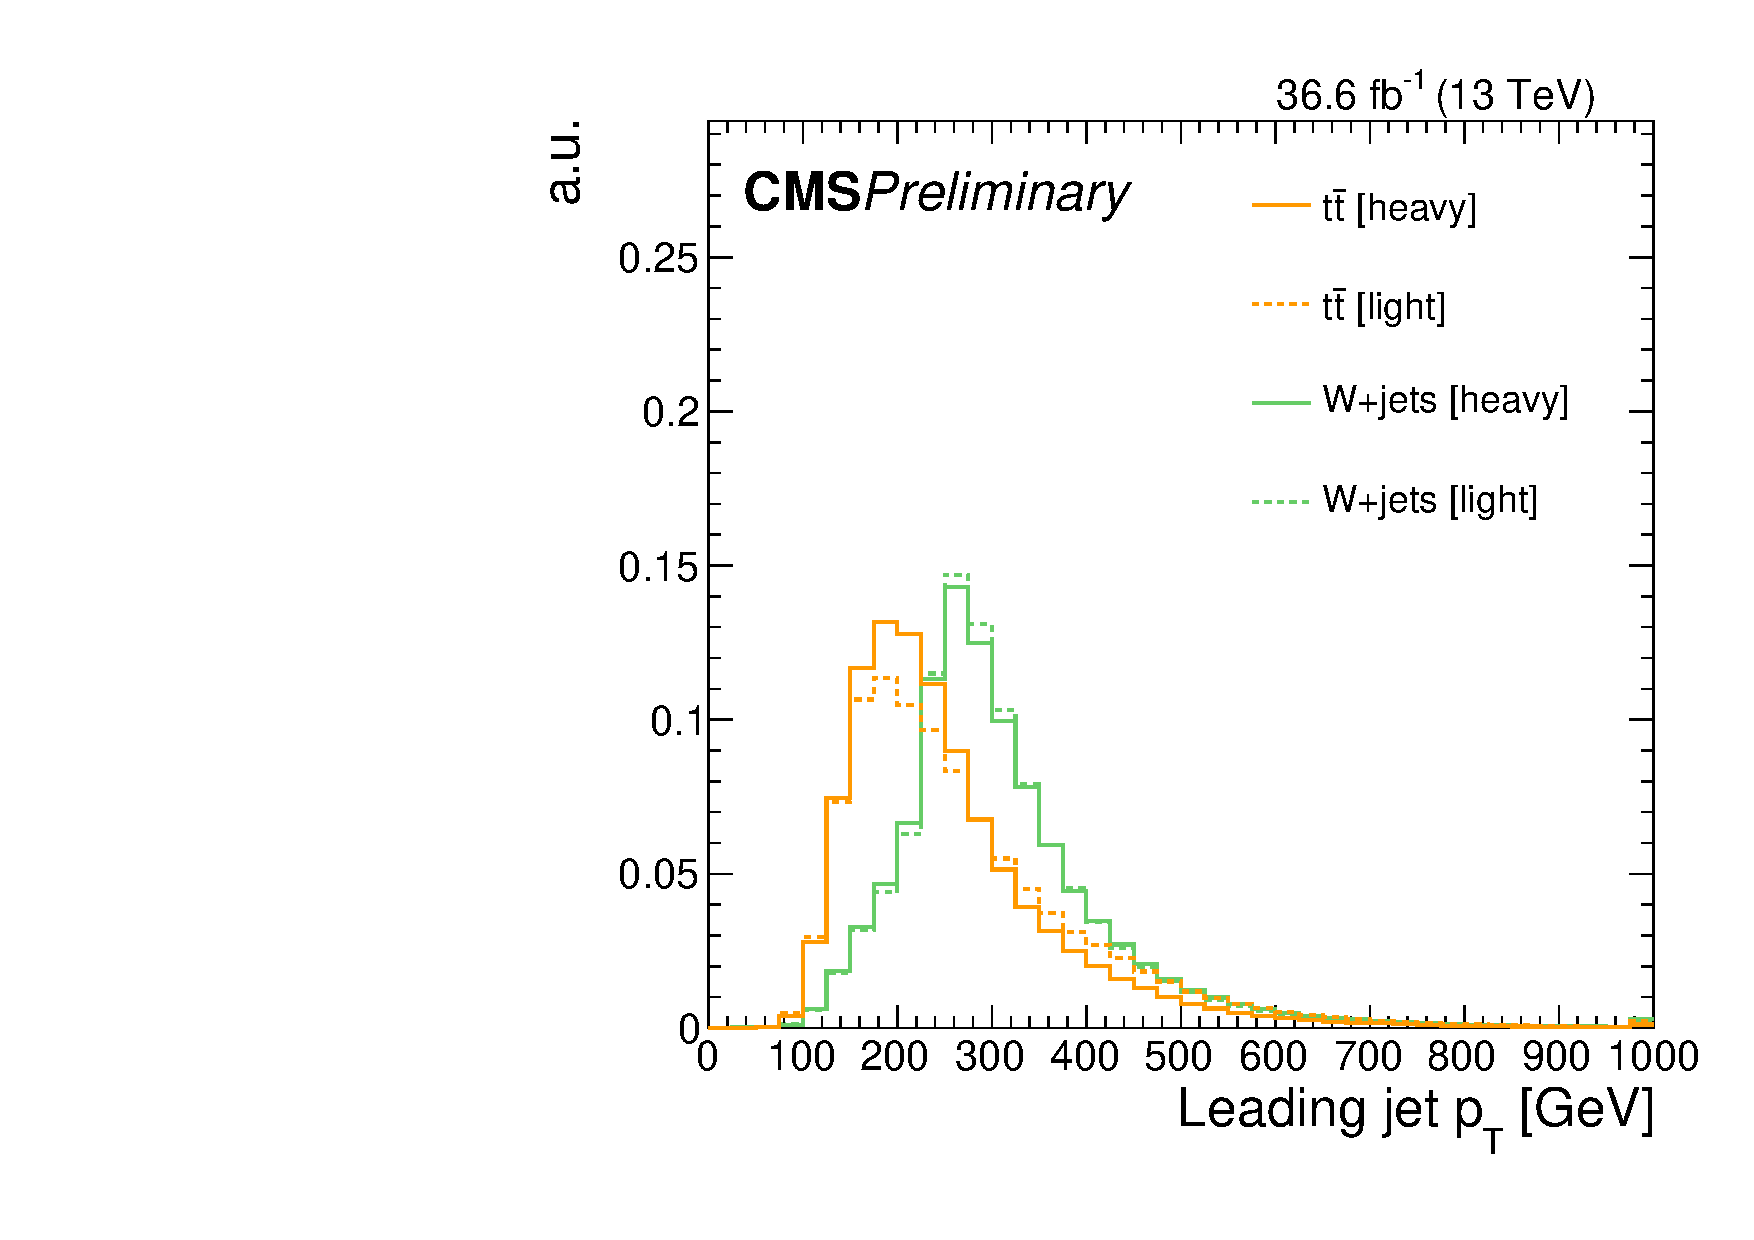
\includegraphics[width=0.49\textwidth]{figures/btag_eff/jet1Pt.pdf}
  \caption{\pt spectra of the leading AK4 jet in $t\bar{t}$ and $W$+jets MC events, after a basic selection ($U>200~\GeV$, fat jet $\pt>200~\GeV$) is applied.
  The shapes are split based on whether the jet is matched to a truth-level $b$ or $c$ (heavy) or not (light).
  In all cases, the bulk of the spectra are well within the range supported by the POG scale factors and uncertainties. }
  \label{fig:bjetspectra}
\end{figure}

As recommended by the BTV POG, we derive the MC efficiency for $b$-tagging jets in the phase space used by this analysis.
The efficiencies are derived using the $t\bar{t}$ Monte Carlo sample and applying a preselection of $U>200~\GeV$.
The jets are split into three categories: $b$ jets (matched to a truth $b$), $c$ jets (matched to a truth $c$), or light-flavor jets (unmatched).
Figure~\ref{fig:btageffs} shows the efficiencies as a function of the reconstructed jet $p_{T}$ and $\eta$

\begin{figure}[htbp]
  \centering
  \subfigure[Light-flavor jets]{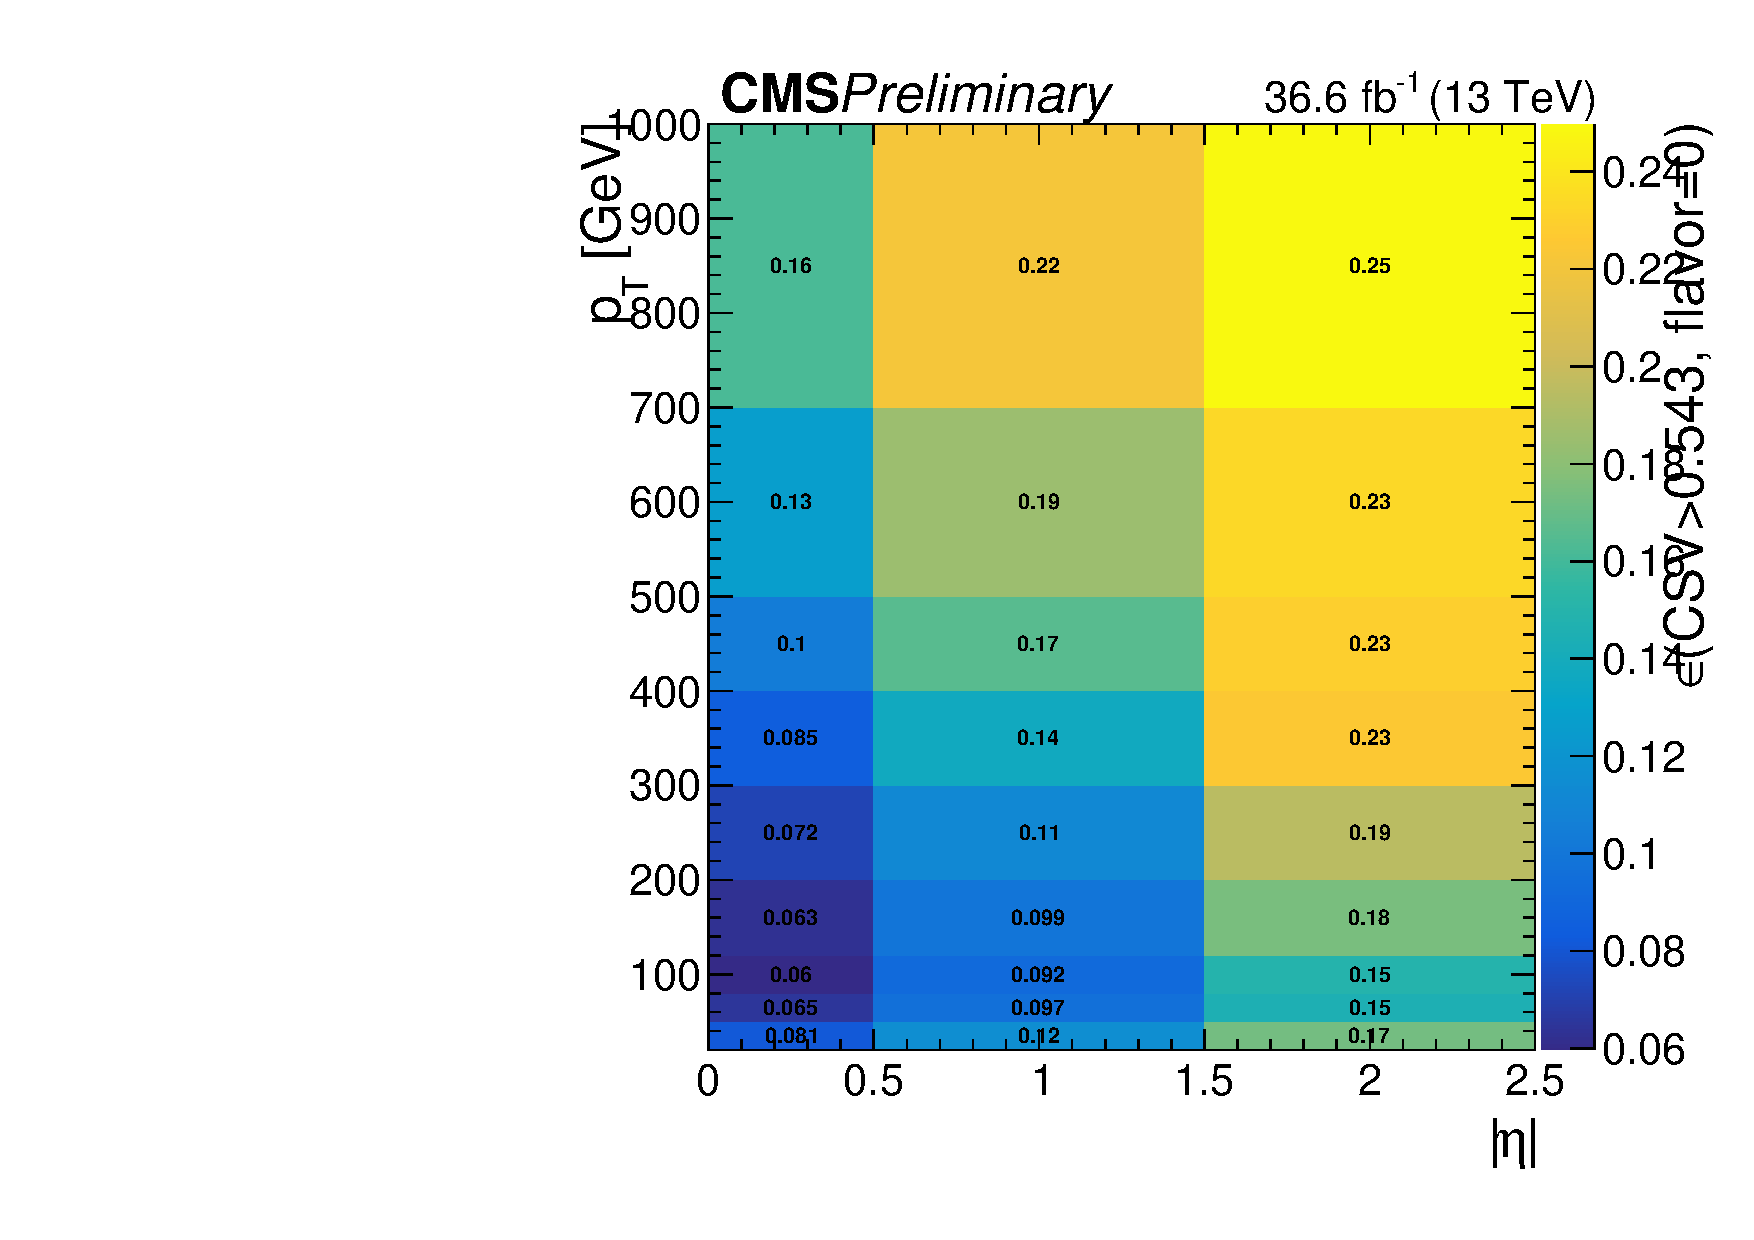
\includegraphics[width=0.33\textwidth]{figures/btag_eff/btag_eff_LWP_flav0.pdf}}
  \subfigure[$c$ jets]{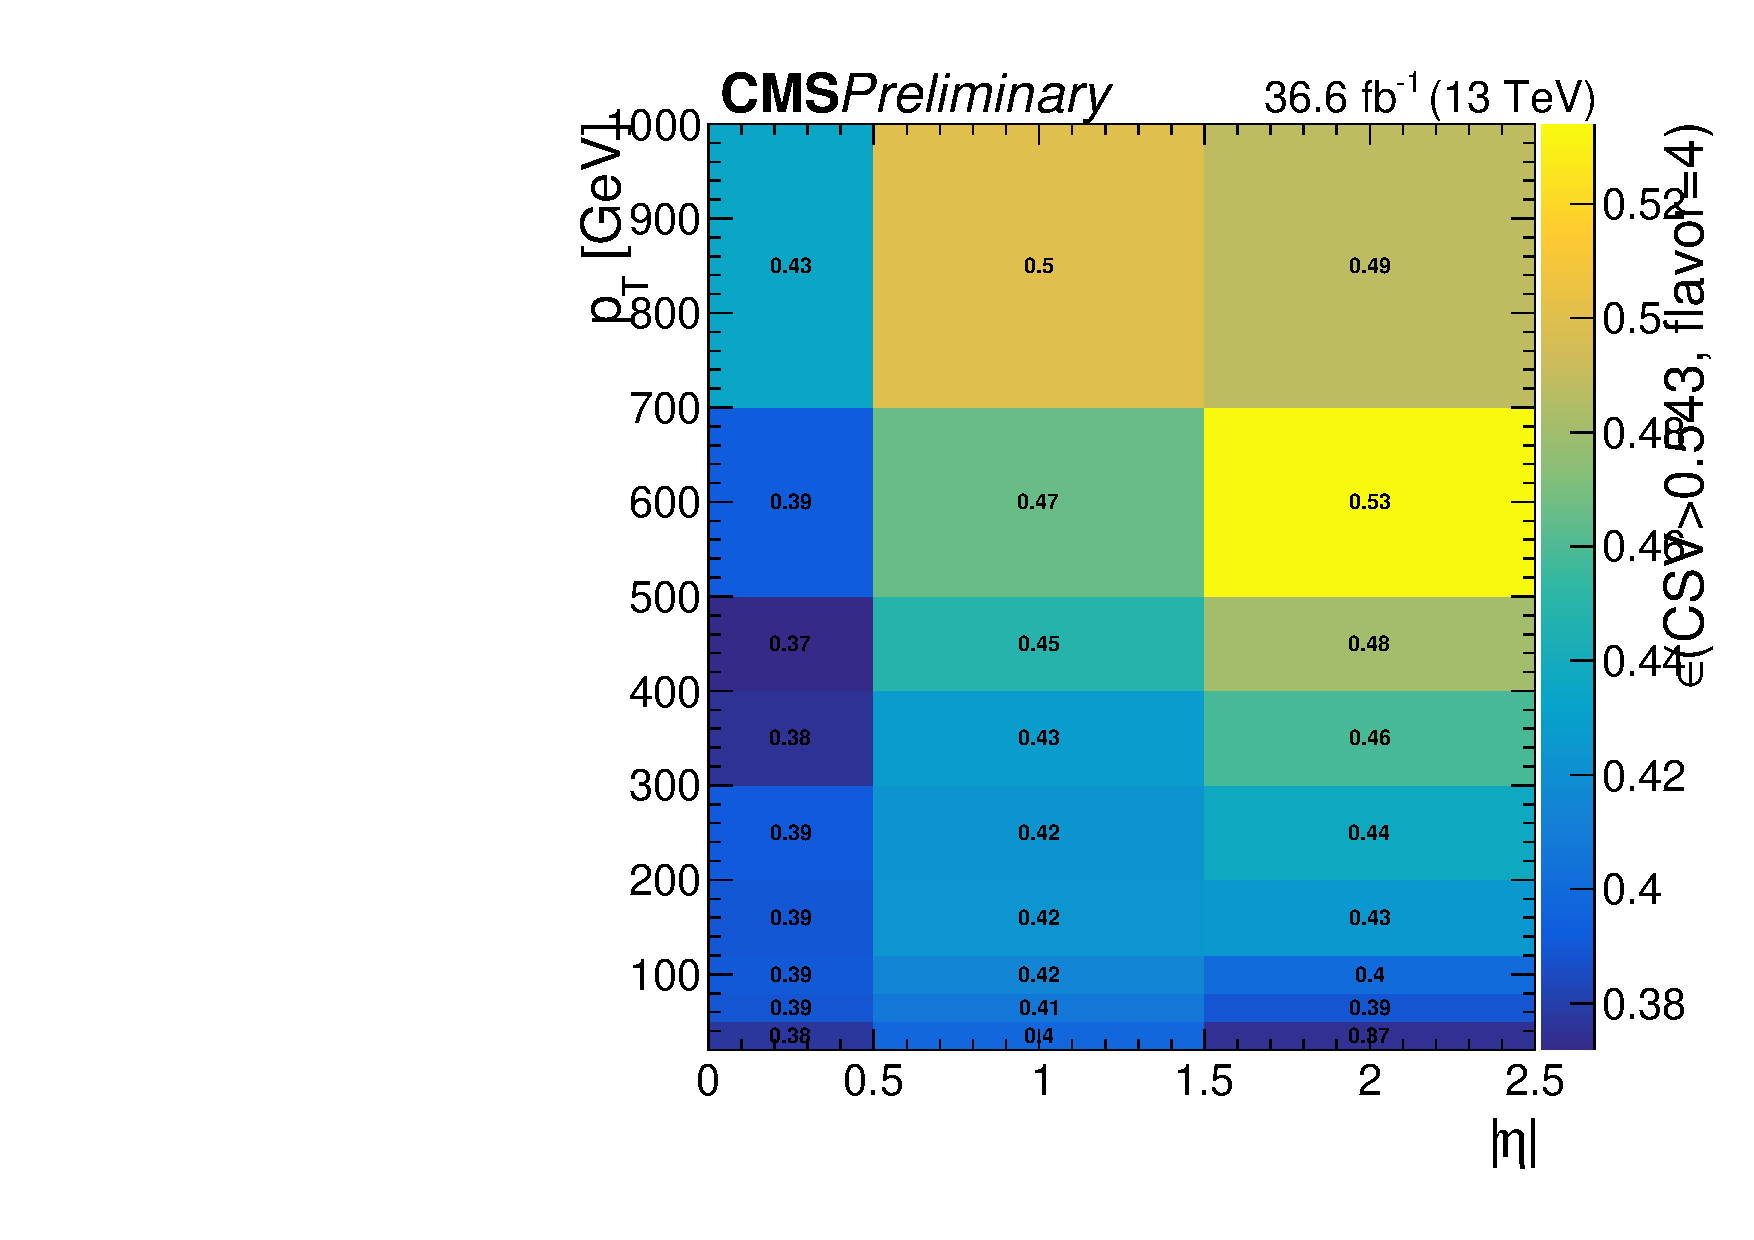
\includegraphics[width=0.33\textwidth]{figures/btag_eff/btag_eff_LWP_flav4.pdf}}
  \subfigure[$b$ jets]{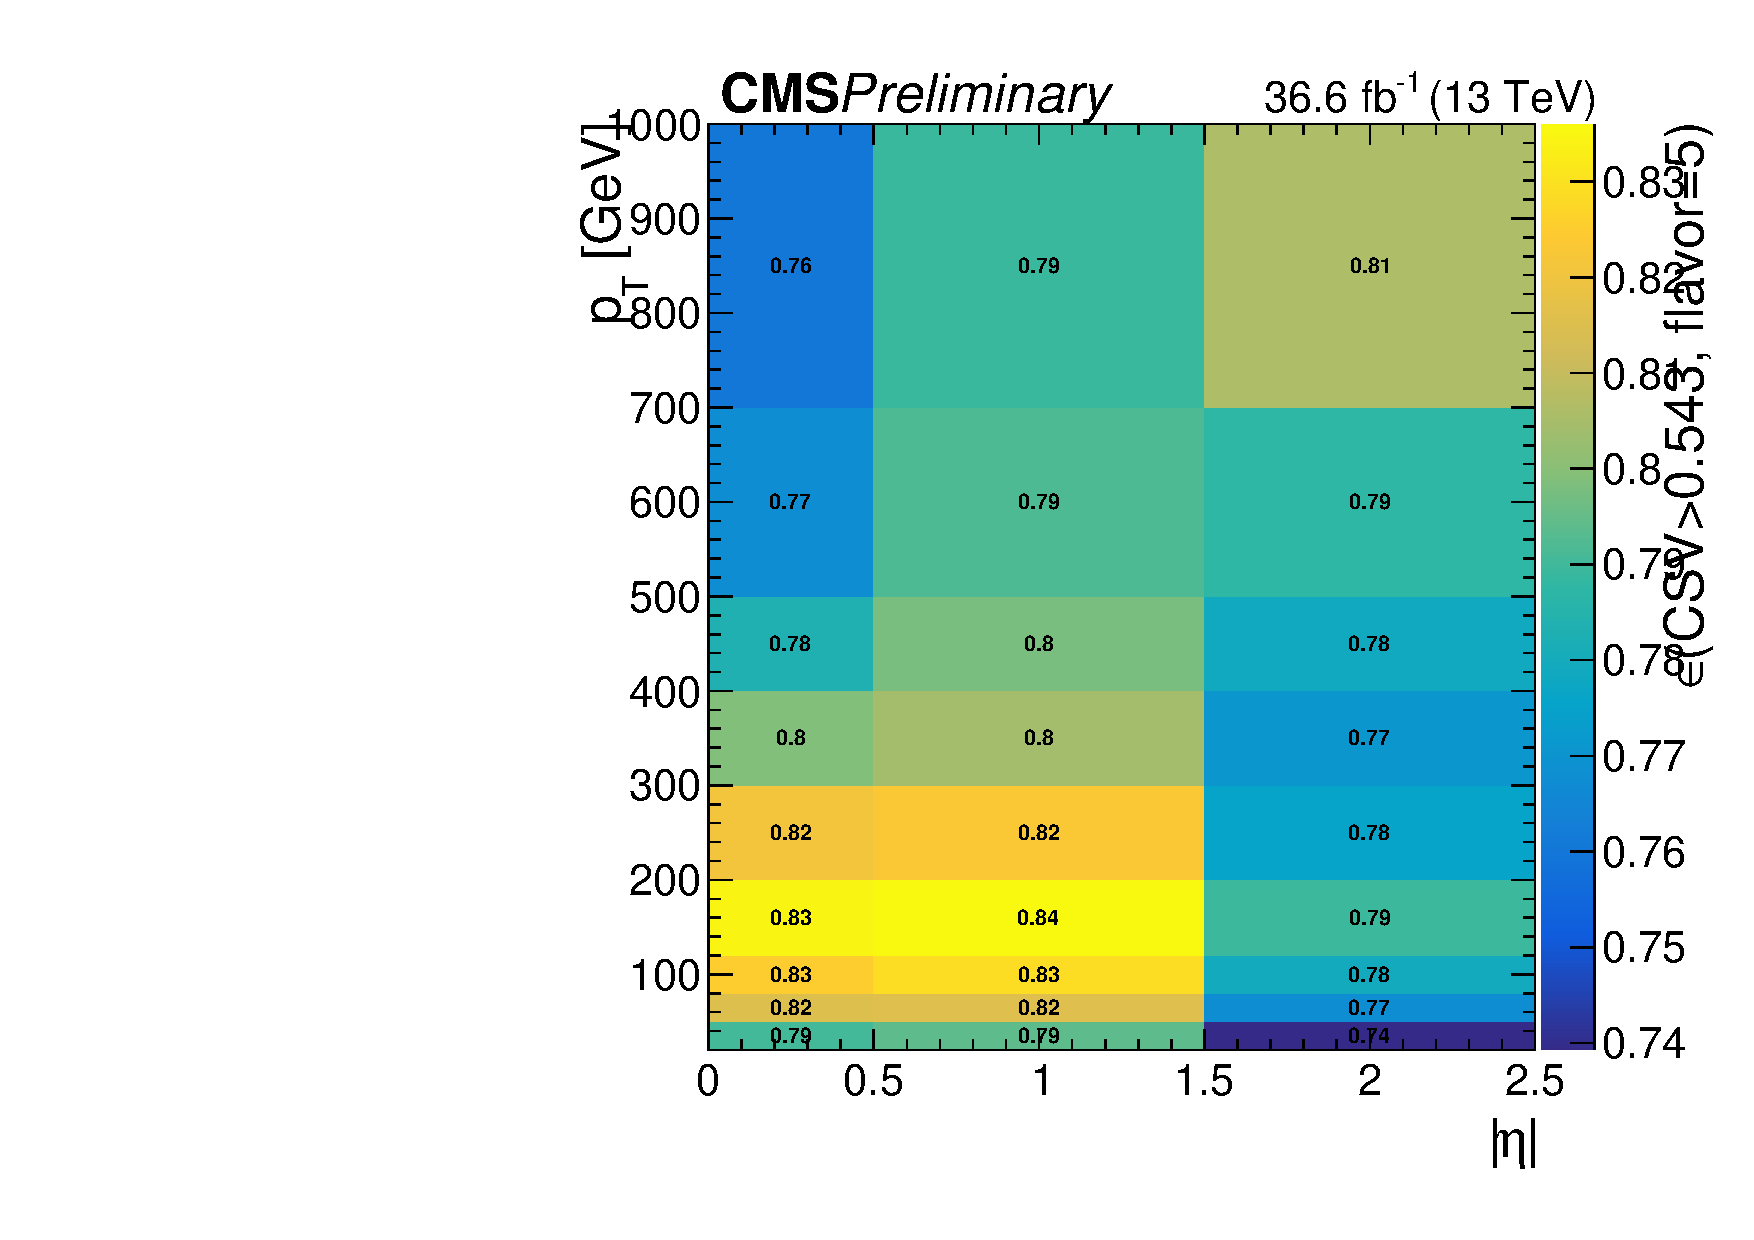
\includegraphics[width=0.33\textwidth]{figures/btag_eff/btag_eff_LWP_flav5.pdf}}
  \caption{$b$-tagging efficiency in the analysis phase space ($U>200~\GeV$). The efficiency is shown in three cases, depending on the truth flavor of the jet.}
  \label{fig:btageffs}
\end{figure}

\subsection{Lepton Efficiency Scale Factors}\label{sec:lep}
We apply data-to-MC scale factors to events in the control regions used in the analysis. These data-to-MC scale factors are derived from the efficiencies that are measured for the electron and muon selections in both data and simulation. The uncertainty on the lepton efficiency scale factor is correlated between the single muon/electron and dimuon/dielectron control regions. There are uncertainties for:
\begin{itemize}
  \item Electron ID and tracking (1\% and 0.5\% per lepton leg, respectively)
  \item Muon ID and tracking (1\% and 0.5\% per lepton leg, respectively)
  \item Tau veto (3\%)
\end{itemize}
A more thorough description of the lepton uncertainties we use are described in~\cite{CMS_AN_2016-473}.

\subsection{Trigger Efficiencies}\label{sec:trigeff}
Single-electron triggers are used to select events with electrons.
The efficiencies of these triggers in data are parametrized as a function of the electron \pt and applied to MC.
The derivation of these efficiencies is described in~\cite{CMS_AN_2016-473}.

\ETmiss triggers are used to select events with real \ETmiss or muons.
The efficiency is parametrized as a function of the hadronic recoil $U$ in such events.
More specifically, it is a function of \ETmiss computed without muons.
However, in the monojet analysis~\cite{CMS_AN_2016-473}, it was found that the efficiency has a small dependence on the number of muons in the event.
The effect comes from muons faking jets in the HLT, lowering the efficiency of the trigger.
At $U=200~\GeV$, the effect is small ($\sim2.5\%$), and decreases at larger $U$. Since we are operating in the realm of $U > 250~\GeV$, this uncertainty is not applicable.
%To account for this difference, a shape uncertainty is applied to all transfer factors into the signal region.
The prescription used is the same as in~\cite{CMS_AN_2016-473}.

\subsection{QCD Normalization Uncertainty}

In this analysis, the QCD background is estimated directly from Monte Carlo simulation in all regions. A $100\%$ uncertainty is applied to the normalization of the QCD. This uncertainty is correlated between regions with the same source of the fake. That is, one uncertainty is applied to QCD in the signal region, a separate uncertainty is applied to QCD in muon control regions, and similarly for electrons. The $100\%$ uncertainty is estimated by looking in a QCD-enriched region:
\begin{itemize}
  \item Veto electrons, muons, taus, photons
  \item Require $\MET>200~\GeV$
  \item Require $\min\Delta\phi(\MET,\text{jet})<0.1$
\end{itemize}
The $\MET$ distribution of this region is shown in Figure~\ref{fig:qcdcr}. The disagreement between data and simulation is at most $50\%$. We double this difference between data and Monte Carlo and use it as the uncertainty on the normalization of QCD.

\begin{figure}[htbp]
  \centering
        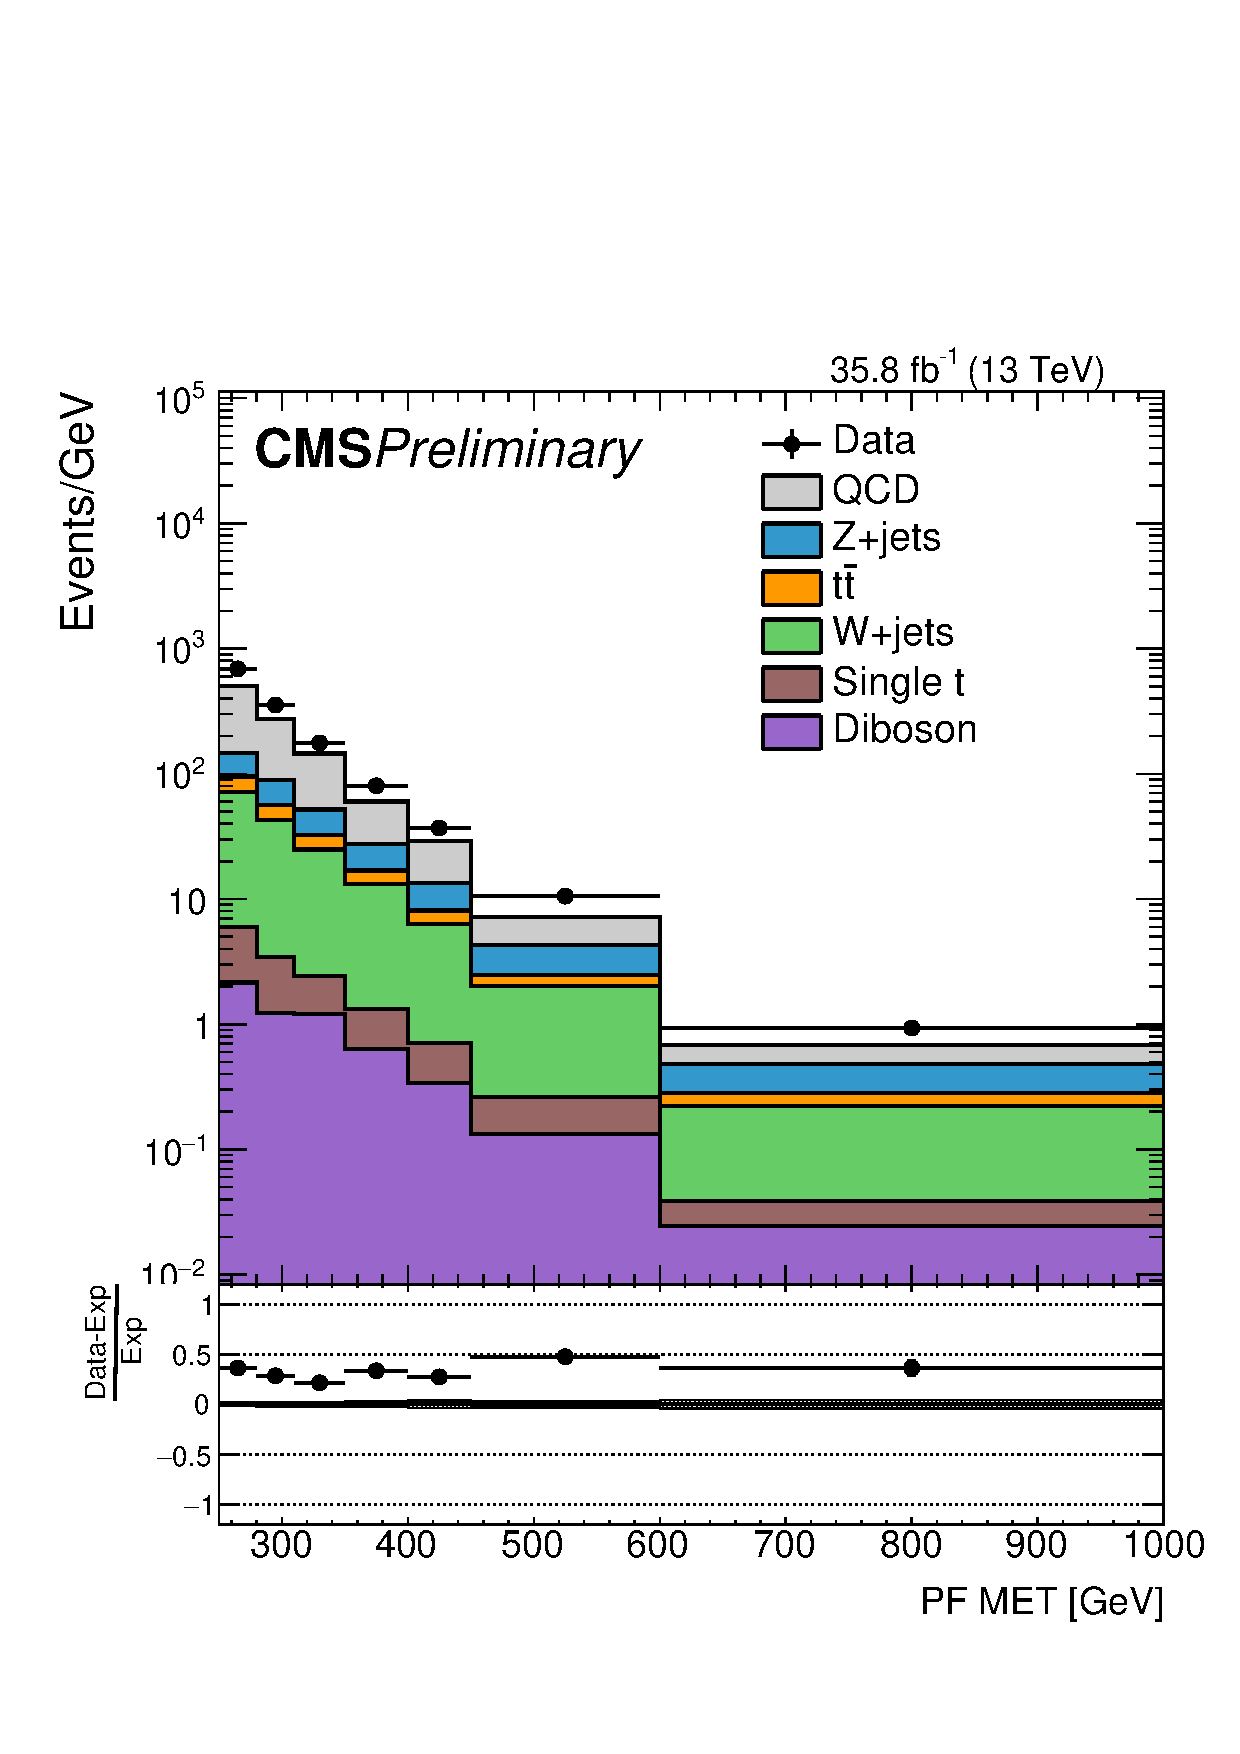
\includegraphics[width=0.6\textwidth]{figures/prefit/onefatjet_m50/qcd_pfmet_logy.pdf}
  \caption{Recoil distribution in a QCD-enriched region. Used to validate the $100\%$ normalization uncertainty applied to QCD. The disagreement is at most $50\%$. }
  \label{fig:qcdcr}
\end{figure}

\subsection{Double-b Scale Factor Uncertainties}\label{sec:doublebunc}
 
In Section~\ref{tagging_efficiency} the derivation of double-b signal scale factors and mistag scale factors for the $t\bar{t}$ process are described. For W/Z+jets production, scale factor are measured simultaneously with the signal extraction directly in the final fit. This in-situ calibration is made possible by using events that fail the double-b requirement. 
The mistag scale factor is taken as a correction to the double-b efficiency for W/Z+jets and included in the fit as an unconstrained nuisance. The double-b efficiency estimated on MC is:
\begin{align}
\epsilon^{\mathrm{W/Z+jets~mis-tag}}_{\mathrm{MC}} &=\frac{N^{\mathrm{pass}}_{W/Z+jets}}{N_{W/Z+jets}} ~,
\end{align}
where $N^{\mathrm{pass}}_{W/Z+jets}$ is the yield of W/Z+jets production in the pass signal/control region (double-b tag $> 0.75$). To take into account the variation of such efficiency introduced by the uncertainty on the heavy flavor fraction of W/Z+jets events, two efficiencies are estimated performing the same calculation described above, but with different $N^{\mathrm{pass}}_{W/Z+jets}$ obtained by pushing up and down the heavy flavor fraction. The difference between the up and down efficiency with respect to the central value is taken as a systematic uncertainty.

The mistag scale factor for W/Z+jets production is obtained by imposing 
\begin{align}
N^{\mathrm{total}}_{W/Z+jets} &=N^{\mathrm{pass}}_{W/Z+jets} + N^{\mathrm{fail}}_{W/Z+jets}
\end{align}
considering
\begin{align}
N^{\mathrm{pass}}_{W/Z+jets} &= \epsilon^{\mathrm{W/Z+jets~mis-tag}}_{\mathrm{data}}\times N^{\mathrm{total}}_{W/Z+jets} &= SF^{\mathrm{W/Z+jets~mis-tag}}_{pass}\times \epsilon^{\mathrm{W/Z+jets~mis-tag}}_{\mathrm{MC}}\times N^{\mathrm{total}}_{W/Z+jets}
\end{align}
and deriving $N^{\mathrm{fail}}_{W/Z+jets}$ as
\begin{align}
N^{\mathrm{fail}}_{W/Z+jets} = N^{\mathrm{total}}_{W/Z+jets}\times (1 - SF^{\mathrm{W/Z+jets~mis-tag}}_{pass}\times \epsilon^{\mathrm{W/Z+jets~mis-tag}}_{\mathrm{MC}})
\end{align}
so that $SF^{\mathrm{W/Z+jets~mis-tag}}_{fail}$ can be expressed in terms of $SF^{\mathrm{W/Z+jets~mis-tag}}_{pass}$ as
\begin{align}
SF^{\mathrm{W/Z+jets~mis-tag}}_{fail} = \frac{1 - SF^{\mathrm{W/Z+jets~mis-tag}}_{pass}\times \epsilon^{\mathrm{W/Z+jets~mis-tag}}_{\mathrm{MC}}}{1 - \epsilon^{\mathrm{W/Z+jets~mis-tag}}_{\mathrm{MC}}}
\end{align}

making $SF^{\mathrm{W/Z+jets~mis-tag}}_{pass}$ the only parameter to be extracted in the fit together with the overall W/Z+jets normalizations. By splitting each control region in pass and fail we have two independent control samples used to constrain two unknowns. The $SF^{\mathrm{W/Z+jets~mis-tag}}_{pass}$ are simultaneously applied to the W/Z+jets processes in signal region, included as extArg in the datacards and measured by combine when running the signal extraction. 

A similar approach is used for the $t\bar{t}$ mistag SF, where the independent measurement described in Section~\ref{mistag_efficiency} is used as prior for the central value of the $SF^{t\bar{t}\mathrm{~mis-tag}}_{pass}$ nuisance and the measured uncertainty as its prior uncertainty in the fit. In this case the efficiency is fixed, since no fluctuation is introduced by any effect like the varying heavy flavor fraction for W/Z+jets.

The exact values for the efficiencies going into the fit and the values of the scale factors extracted from it are as follows: 

Prefit: $\epsilon^{\mathrm{W+jets~mis-tag}}_{\mathrm{MC}}=0.0316\pm 0.00126$, $\epsilon^{\mathrm{Z+jets~mis-tag}}_{\mathrm{MC}}=0.0346\pm 0.00174$, $\epsilon^{t\bar{t}}_{\mathrm{MC}}=0.1678\pm 0.0$

Postfit: $\epsilon^{\mathrm{W+jets~mis-tag}}_{\mathrm{MC}}=0.0316\pm 0.00124$, $\epsilon^{\mathrm{Z+jets~mis-tag}}_{\mathrm{MC}}=0.0346\pm 0.00171$, $\epsilon^{t\bar{t}}_{\mathrm{MC}}=0.1678\pm 0.0$

SF: $SF^{\mathrm{W+jets~mis-tag}}_{pass}=1.21\pm0.24$, $SF^{\mathrm{Z+jets~mis-tag}}_{pass}=1.12\pm0.15$ ,$SF^{t\bar{t}~\mathrm{mis-tag}}_{pass}=1.033\pm0.058$


%In addition to these global SFs adjusting the overall pass/fail ratios, we apply a \pt-dependent shape uncertainty on the transfer factors from any fail CR to the SR. These are uncorrelated between W+jets and Z+jets, but are correlated across all recoil bins and address potential systematic effects with a residual \pt dependence, such as a varying heavy flavor contribution across the bins or a varying tagging efficiency for QCD jets, as is suggested by the studies performed in~\cite{boostedhiggs}. The uncertainties on the four recoil bins are 0\%, 2\%, 4\%, and, respectively, 8\%.

As studies have shown, tying together the W+jets and Z+jets backgrounds to have one floating SF and one \pt-dependent component for V+jets does not impact our result significantly, and we prefer to leave them as separate parameters/nuisances, as there is a good physics motivation (different heavy flavor content and production mechanisms for W or Z) to do so.


\subsection{Additional Uncertainties}\label{sec:add}
Additional rate uncertainties on the luminosity measurement (2.5\%) and on the theoretical cross section for MC-driven processes are included and correlated through the different samples. 
We apply a $5\%$ rate uncertainty to cover MET bin migration, as done in ~\cite{CMS_AN_2016-473}. 
It is derived by propagating the jet energy scale and resolution uncertainties to the MET~\cite{JEC_TWIKI,JER_TWIKI}, and is the signal uncertainty on the MET.
An additional $4\%$ rate uncertainty is considered to cover the effect of the CA15 jet energy scale. 
This is derived by propagating the AK8 jet energy scale uncertainties from the POG, with a factor of two added to cover the extrapolation from AK8 to CA15.
These rate uncertainties are only applied to processes that are predicted by non-data-driven methods.
